\clearpage
\section{Customer Relationship Management}

Das CRM (Customer Relationship Management) ermöglicht Ihnen effizient Veranstaltungen (Anlässe, Präsentationen und Schulungen) zu koordinieren. Es unterstützt Sie bei der Einladung, dem Verwalten von Anmeldungen, Versenden von Erinnerungen und dem Erstellen von Teilnehmerlisten.

\vspace{\baselineskip}

Für Ihre Veranstaltung erstellen Sie über eine Webseite eine Einladung in Form eines Online-Flyers mit den wichtigsten Angaben zum Anlass, Eckdaten wie Termin, Zeit, Bemerkungen und Weiteres. Die Email-Einladung, welche auf diese Einladungsseite verweist, versenden Sie aus dem CRM an eine gewünschte Personengruppe. Die Eingeladenen können über diese Webseite Ihre Anmeldung für den Anlass durchführen (mittels Klick) oder falls notwendig zu Beginn oder später Ihre Entschuldigung einreichen. Sie als Organisator haben jederzeit den Überblick über die versendeten Einladungen und deren Status. Sie sehen sofort wie viele Personen sich bereits an- oder abgemeldet haben. \\

Schliesslich können Sie eine Teilnehmerliste exportieren und können auf diese Weise das Resultat Ihrer Einladung auswerten oder weiterreichen.

\vspace{\baselineskip}

Das CRM ist in zwei Teile gegliedert: 
\begin{compactitem}
\item
\textbf{Veranstaltungstypen:} Hier legen Sie die verschiedenen Arten von Veranstaltungen fest (bspw. Jahresrückblick, Neuheiten-Präsentation etc.).
\item
\textbf{Veranstaltungen:} Unter diesem Menüpunkt werden die konkreten Veranstaltungen geplant. Nach dem Anlegen einer Veranstaltung haben Sie die Möglichkeit, die Einladungswebseite (Online-Flyer) zu gestalten.
\end{compactitem}

\vspace{\baselineskip}

Zudem können \textbf{Teilnehmerlisten} erfasst werden. Weitere Informationen zum Erstellen von vordefinierten Teilnehmerliste siehe Kapitel \ref{bkm:Ref2018072301}.

\pagebreak
\subsection{Veranstaltungstypen}

\begin{wrapfigure}[7]{l}{6.5cm}   % [x] Wie manche Zeile soll sich um die Grafik "brechen"
  \vspace{-35pt}      % Grundwert war 20; mit 30 schön oben beim Text ausgerichtet
  \begin{center}
    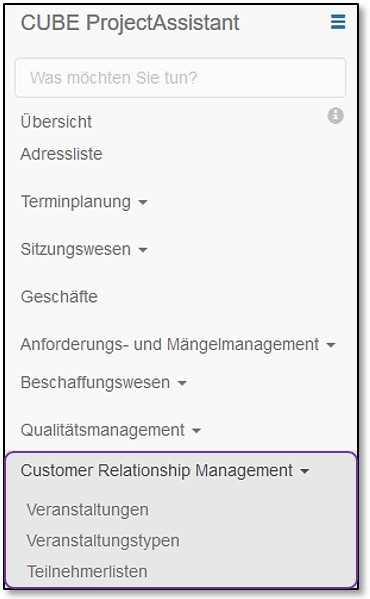
\includegraphics[width=1\linewidth]{../chapters/10_CRM/pictures/10-1-1_Menu_CRM.jpg}
  \end{center}
  \vspace{-20pt}
  \caption{Das CRM Menü}
  \vspace{-10pt}
\end{wrapfigure}

\textbf{Übersicht:} Klicken Sie im Menü links auf 'Customer Relationship Management' und den Unterpunkt Veranstaltungstypen.\\


\textbf{Hinweis:} Bevor Sie mit dem Erstellen einer Veranstaltung beginnen, erfassen Sie den oder die gewünschten Veranstaltungstyp/en. 

\vspace{8cm}

Die Übersicht der Veranstaltungstypen öffnet sich:

\begin{figure}[H]
\center{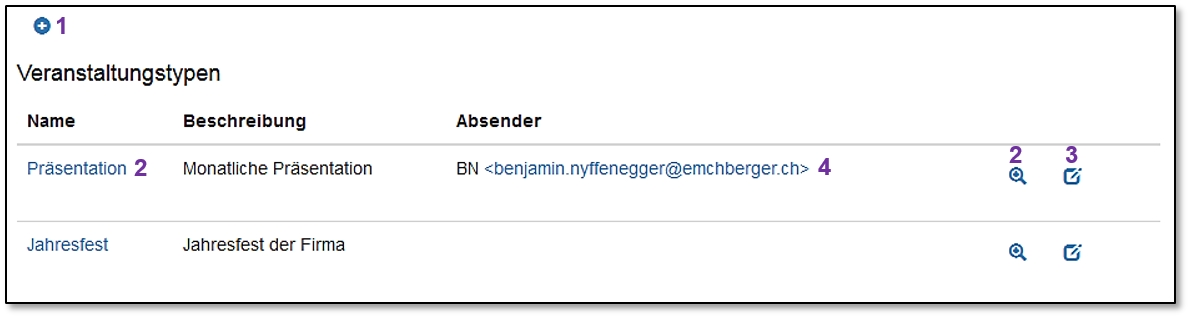
\includegraphics[width=1\linewidth]{../chapters/10_CRM/pictures/10-1_VeranstTyp_Uebersicht.jpg}}
\caption{Übersicht Veranstaltungstypen}
% \label{fig:speciation}
\end{figure}

Sie sehen alle erfassten Veranstaltungstypen. Mit Klick auf das Plussymbol 
\includegraphics[height=12pt]{/Icons/Plussymbol.jpg} \col{(1)} können Sie einen neuen Veranstaltungstyp erstellen. Mit Klick auf den entsprechenden Veranstaltungstyp \col{(2)} oder auf das Lupensymbol 
\includegraphics[height=12pt]{/Icons/Lupe.jpg} \col{(2)} können Sie die Details eines Veranstaltungstypen betrachten. Um einen Eintrag zu bearbeiten, klicken Sie auf das Bearbeiten-Symbol 
\includegraphics[height=12pt]{/Icons/Bearbeiten.jpg} \col{(3)}. Wurde eine Absender-Emailadresse hinterlegt, können Sie mit Klick auf diese \col{(4)} eine Email versenden. Wählen Sie das gewünschte Emailprogramm aus.

\subsubsection{Neue Veranstaltungstypen anlegen}

\begin{figure}[H]
\center{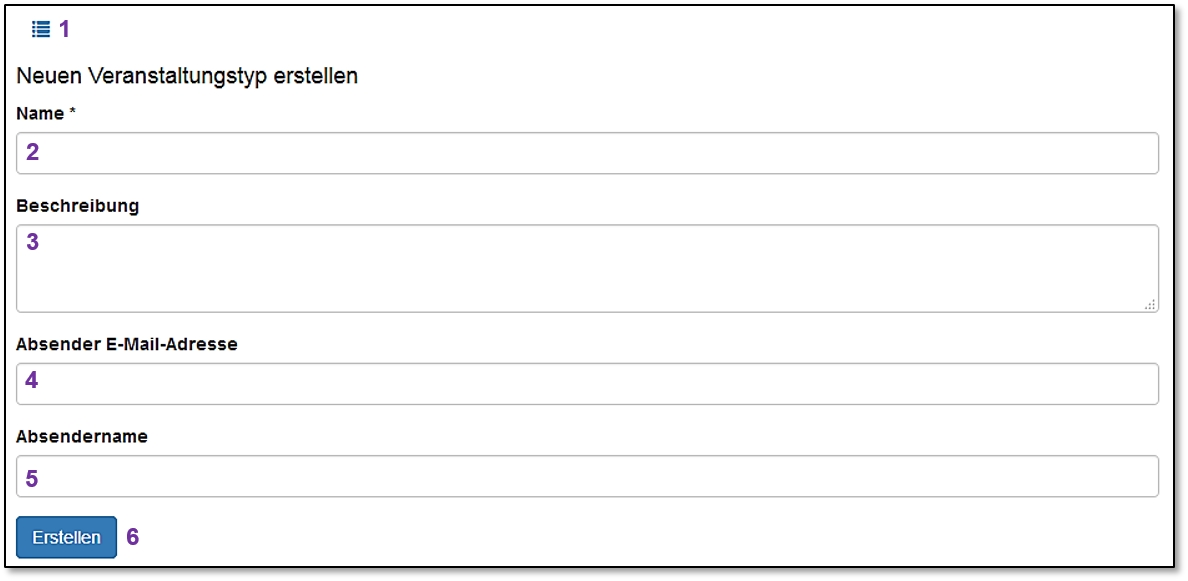
\includegraphics[width=1\linewidth]{../chapters/10_CRM/pictures/10-1_VeranstTyp_erstellen.jpg}}
\caption{Neue Veranstaltungstypen erstellen}
% \label{fig:speciation}
\end{figure}

Mit Klick auf das Listensymbol 
\includegraphics[height=12pt]{/Icons/Listensymbol_zurueck.jpg} \col{(1)} kehren Sie jederzeit auf die Übersicht zurück.\\
Geben Sie einen aussagekräftigen Namen \col{(2)} für den gewünschten Veranstaltungstyp ein (Dies ist ein Pflichtfeld und muss als einziges ausgefüllt werden). Unter 'Beschreibung' \col {(3)} können Sie den Veranstaltungstyp präziser beschreiben. Sie haben die Möglichkeit, eine Absender-Emailadresse \col{(4)} und einen Absendernamen \col{(5)} zu hinterlegen. Wird eine Emailadresse eingetragen, können Sie in der Übersicht mit Klick auf die Emailadresse direkt eine Email versenden. Nach den Eingaben schliessen Sie den Vorgang mit 'Erstellen' \col{(6)} ab.

\subsubsection{Bestehende Veranstaltungstypen betrachten und bearbeiten}

\begin{wrapfigure}[12]{l}{6.5cm}   % [x] Wie manche Zeile soll sich um die Grafik "brechen"
  \vspace{-35pt}      % Grundwert war 20; mit 30 schön oben beim Text ausgerichtet
  \begin{center}
    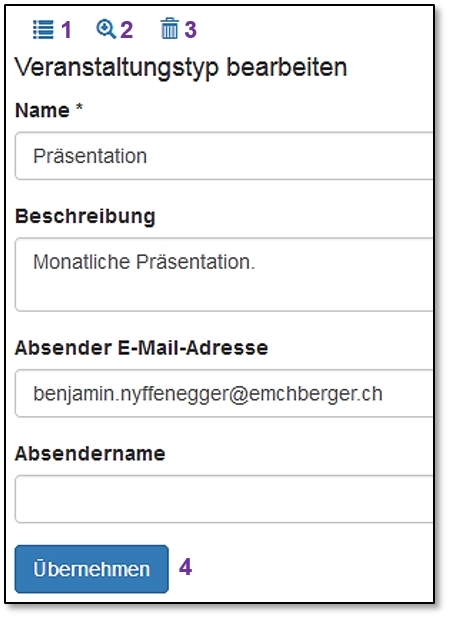
\includegraphics[width=1\linewidth]{../chapters/10_CRM/pictures/10-1-2_Veranstaltungstyp_bearbeiten.jpg}
  \end{center}
  \vspace{-20pt}
 % \caption{Veranstaltungstyp bearbeiten}
  \vspace{-10pt}
\end{wrapfigure}

Klicken Sie in der Übersicht der Veranstaltungstypen auf das Bearbeiten-Symbol 
\includegraphics[height=12pt]{/Icons/Bearbeiten.jpg}, um einen bereits erstellen Eintrag zu ändern. Die Maske mit den ausgefüllten Feldern wird geöffnet. Schliessen Sie diesen Vorgang mit Klick auf 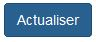
\includegraphics[height=12pt]{/Icons/B_Uebernehmen.jpg} \col{(4)} ab. Die Maske wird nicht automatisch geschlossen. Mit Klick auf das Listensymbol 
\includegraphics[height=12pt]{/Icons/Listensymbol_zurueck.jpg} \col{(1)} kehren Sie zur Übersicht zurück. Sie können mittels dem Lupensymbol 
\includegraphics[height=12pt]{/Icons/Lupe.jpg} \col{(2)} den Eintrag betrachten. Im Bearbeitungsmodus haben Sie zudem die Möglichkeit, mittels Klick auf das Mülltonnensymbol 
\includegraphics[height=12pt]{/Icons/Muelltonne.jpg} \col{(3)} einen Eintrag zu löschen.

\vspace{\baselineskip}

\subsection{Veranstaltungen}

Klicken Sie links im Menü unter 'Customer Relationship Management' den Unterpunkt Veranstaltungen. Sie erhalten die Übersicht über alle bestehenden Veranstaltungen:

\begin{figure}[H]
\center{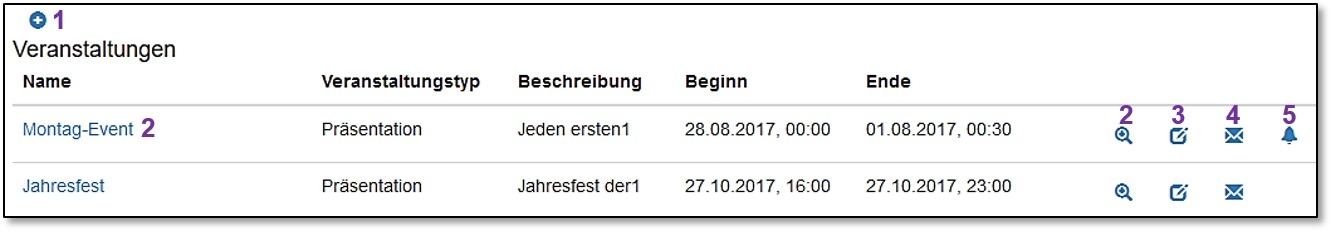
\includegraphics[width=1\linewidth]{../chapters/10_CRM/pictures/10-2_Veranstaltungen_Uebersicht.jpg}}
\caption{Übersicht Veranstaltungen}
% \label{fig:speciation}
\end{figure}

Mit Klick auf das Plussymbol 
\includegraphics[height=12pt]{/Icons/Plussymbol.jpg} \col{(1)} können Sie neue Veranstaltungen hinzufügen. Wenn Sie auf den blauen Veranstaltungstitel oder das Lupensymbol 
\includegraphics[height=12pt]{/Icons/Lupe.jpg} \col{(2)} klicken, können Sie einen Eintrag anschauen. Um eine Veranstaltung zu bearbeiten, klicken Sie auf das Bearbeiten-Symbol 
\includegraphics[height=12pt]{/Icons/Bearbeiten.jpg} \col{(3)}. Mit Klick auf das Mailsymbol 
\includegraphics[height=12pt]{/Icons/Briefsymbol.jpg} \col{(4)} gelangen Sie in den Versandmodus, in welchem Sie die Email-Vorlage bearbeiten können. Wurde bei Veranstaltungen bereits eine Einladung verschickt, können Sie mit dem Glocken-Symbol 
\includegraphics[height=12pt]{/Icons/Glocke.jpg} \col{(5)} eine Erinnerung versenden, resp. gelangen Sie auf die Erinnerungsseite.

% \pagebreak
\subsubsection{Neue Veranstaltungen anlegen}

Klicken Sie auf das Plussymbol 
\includegraphics[height=12pt]{/Icons/Plussymbol.jpg} in der Veranstaltungsübersicht, um eine neue Veranstaltung anzulegen.

\begin{wrapfigure}[15]{l}{6.5cm}   % [x] Wie manche Zeile soll sich um die Grafik "brechen"
  \vspace{-30pt}      % Grundwert war 20; mit 30 schön oben beim Text ausgerichtet
  \begin{center}
    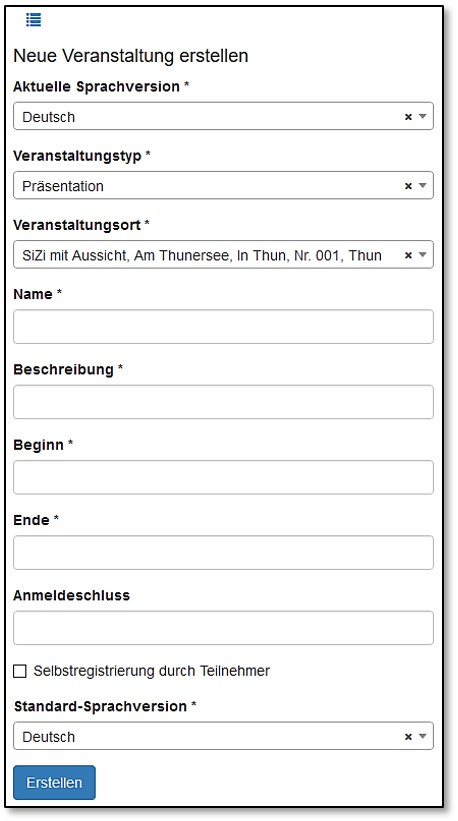
\includegraphics[width=1\linewidth]{../chapters/10_CRM/pictures/10-2-1_NeueVeranstaltung.jpg}
  \end{center}
  \vspace{-20pt}
  % \caption{Neue Veranstaltung anlegen}
  \vspace{-10pt}
\end{wrapfigure}

Die Eingabemaske erscheint. Bei den Feldern 'Veranstaltungstyp' und 'Veranstaltungsort' handelt es sich um Dropdown-Listen. Wählen Sie unter den Einträgen den gewünschten aus.

\vspace{\baselineskip}

\textbf{Hinweis:} Die Veranstaltungsorte müssen vorgängig durch einen Administrator oder berechtigten CUBE PA Superuser in der Konfiguration hinterlegt werden. Bei Fragen können Sie eine Email an den CUBE PA Support senden: {\color{red} cube.support@emchberger.ch}.\\
Die meisten Felder sind Pflichtfelder und müssen ausgefüllt werden. Sind alle Eingaben, gemacht klicken Sie auf den 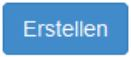
\includegraphics[height=12pt]{/Icons/B_Erstellen.jpg}-Button. Die Veranstaltung wird gespeichert und weitere Optionen werden nun angezeigt:

\vspace{\baselineskip}

\begin{wrapfigure}[18]{l}{6.5cm}   % [x] Wie manche Zeile soll sich um die Grafik "brechen"
  \vspace{-25pt}      % Grundwert war 20; mit 30 schön oben beim Text ausgerichtet
  \begin{center}
    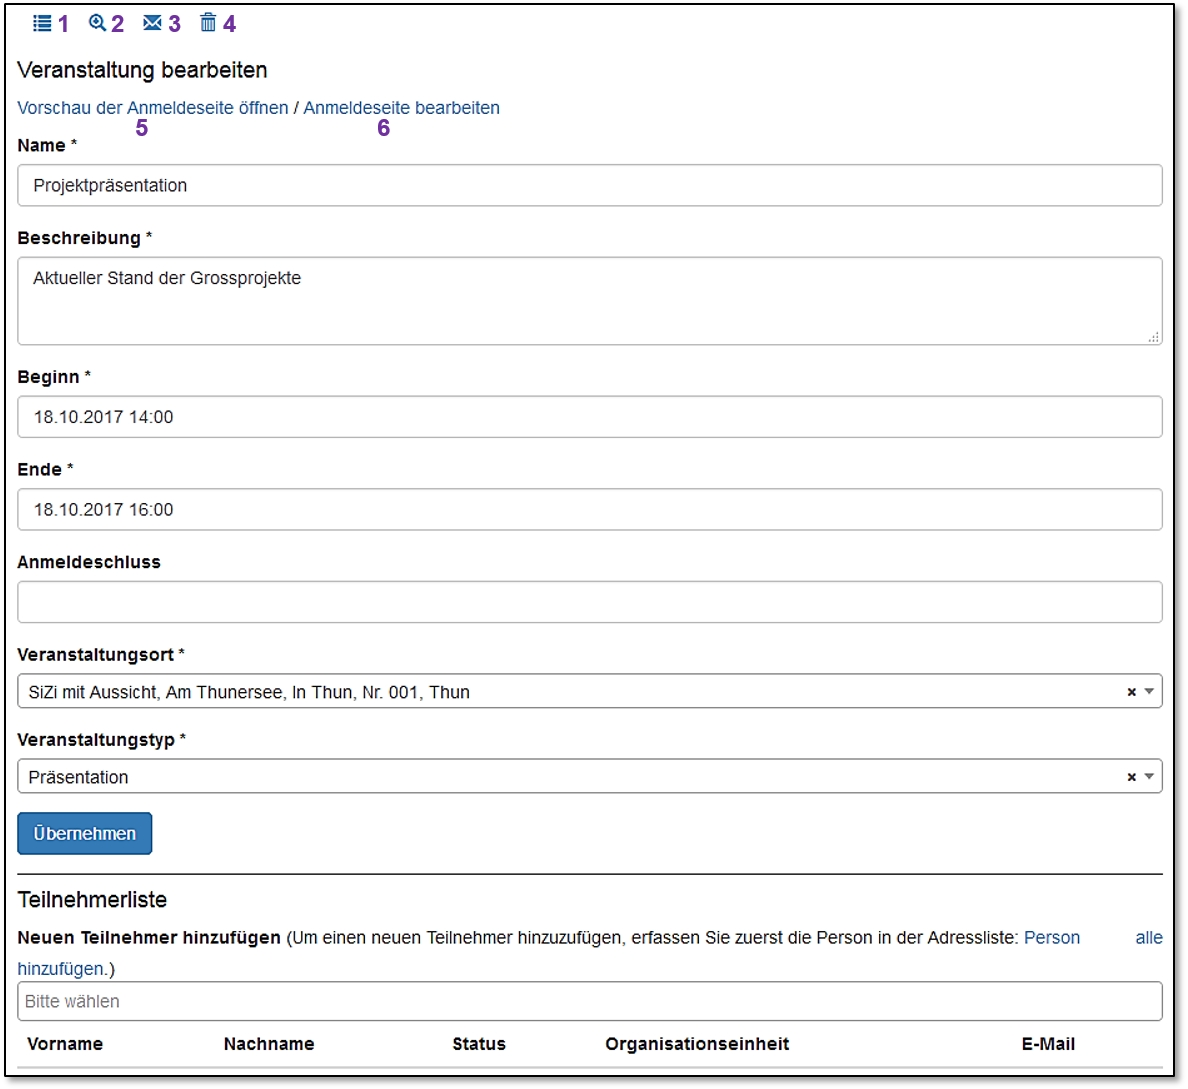
\includegraphics[width=1\linewidth]{../chapters/10_CRM/pictures/10-2-1_NeueVeranstaltung_erweitert.jpg}
  \end{center}
  \vspace{-20pt}
  % \caption{Neue Veranstaltung anlegen - erweiterte Ansicht}
  \vspace{-10pt}
\end{wrapfigure}

Mit Klick auf das Listensymbol 
\includegraphics[height=12pt]{/Icons/Listensymbol.jpg} \col{(1)} kehren Sie zur Veranstaltungsübersicht zurück. Verlassen Sie den Bearbeitungsmodus mit Klick auf die Lupe 
\includegraphics[height=12pt]{/Icons/Lupe.jpg} \col{(2)}. Die Teilnehmerverwaltung erreichen Sie mit Klick auf das Gruppen-Symbol 
\includegraphics[height=12pt]{/Icons/Gruppe.jpg} \col{(3)}. Mehr über die Gruppenverwaltung erfahren Sie in Kapitel \ref{bkm:Ref112017102}. Mittels dem Mailsymbol 
\includegraphics[height=12pt]{/Icons/Briefsymbol.jpg} \col{(4)} wechseln Sie in die Mailvorlagenansicht und mit dem Mülltonnensymbol 
\includegraphics[height=12pt]{/Icons/Muelltonne.jpg} \col{(5)} können Sie die Veranstaltung wieder löschen.\\
Nun haben Sie auch die Möglichkeit, die Einladungsseite (Online-Flyer) zu erstellen. Mit Klick auf den blauen Text 'Anmeldeseite bearbeiten' \col{(7)} gelangen Sie auf die Gestaltungswebseite. Mit Klick auf den blauen Text 'Vorschau der Anmeldeseite öffnen' \col{(6)} können Sie Ihre Einladungsseite ansehen. Mehr dazu im Kapitel \ref{bkm:Ref112017101} (Einladungsseite gestalten).

\vspace{\baselineskip}

\textbf{Mehrsprachigkeit:} Die Einladungen und Erinnerungen sowie die Einladungsseite können aktuell in drei Sprachen (Deutsch, Französisch und Englisch) geschrieben und publiziert werden. Sobald die 'Aktuelle Sprachversion *' umgestellt wird, ändern sich auch die Sprachvorlage für genannte Seiten. 
% Allenfalls Rückfallebene dokumentieren; wird nichts eingestellt, gilt was in der Benutzerverwaltung für eine Person hinterlegt ist... (?)

\vspace{\baselineskip}

\textbf{Selbstregistrierung durch Teilnehmer:} In aller Regel werden Teilnehmer gezielt und persönlich eingeladen. Entsprechend wird die Teilnehmerliste verwendet und die Eingeladenen definiert. Sollen sich jedoch bei einer Veranstaltung auch 'unbekannte' Personen anmelden können und wird beispielsweise ein Mail mit Einladungslink verteilt  (z.B. für Messen), wird diese Option gewählt. Beliebige Personen, welche den Einladungslink erhalten, können sich nun für die Veranstaltung registrieren. Mehr dazu in Kapitel \ref{bkm:Ref2018072302}.

\subsubsection{Teilnehmer verwalten}
\label{bkm:Ref112017102}

\textbf{Hinweis:} Vorgängig müssen Teilnehmer in der Adressliste erfasst werden, damit sie im CRM für die Anmeldung zur Verfügung stehen (es sei denn, Sie wählen bei der Veranstaltung die Option 'Selbstregistrierung durch Teilnehmer' (siehe Kapitel \ref{bkm:Ref2018072302}).

\vspace{\baselineskip}

Die Teilnehmerliste im Überblick:

\begin{figure}[H]
\center{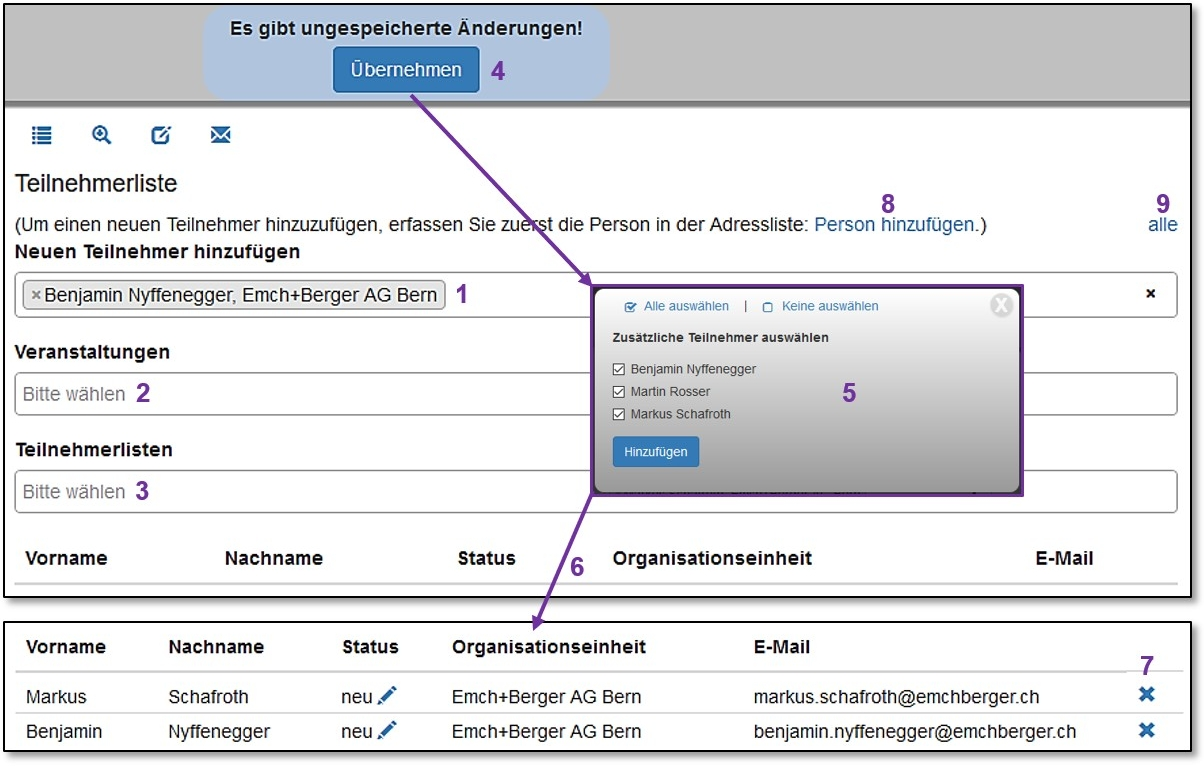
\includegraphics[width=1\linewidth]{../chapters/10_CRM/pictures/crm_Teilnehmerverwaltung.jpg}}
\caption{Teilnehmerliste bearbeiten}
% \label{fig:speciation}
\end{figure}

Neue Teilnehmer können Sie auf verschiedene Weise hinzufügen:
\begin{compactitem}
	\item \textbf{Neuen Teilnehmer hinzufügen}\col{(1)}: Wählen Sie Personen aus, welche im CUBE PA bereits erfasst sind. Falls Sie bei diesem Schritt Personen nicht auffinden, können Sie unter \col{(8)} neue Personen in einem weiteren Browserfenster hinzufügen.
	\item \textbf{Veranstaltungen}\col{(2)}: Wählen Sie eine Veranstaltung aus, welche dieselben Teilnehmer hinterlegt hat. Die Teilnehmer werden übernommen.
	\item \textbf{Teilnehmerlisten}\col{(3)}: Vorgefasste Teilnehmerlisten können hier eingetragen werden. Mehr zu Teilnehmerlisten siehe Kapitel \ref{bkm:Ref2018072301}
\end{compactitem}

\vspace{\baselineskip}

Sobald Sie auf 'Übernehmen' \col{(4)} klicken, wird ein Dialogfenster geöffnet \col{(5)}, in welchem Sie nochmals die ausgewählten Teilnehmer sehen und Anpassungen vornehmen können. Nach Klick auf 'Hinzufügen' werden die ausgewählten Teilnehmer in der Teilnehmerliste übernommen \col{(6)}. Mit dem Kreuzchen-Symbol 
\includegraphics[height=12pt]{/Icons/Kreuzchen_b.jpg} \col{(7)} können Sie Teilnehmer wieder löschen. \\
\textbf{Hinweis:} Teilnehmer können nur gelöscht werden, wenn sie den Status 'neu' haben.

\vspace{\baselineskip}

Wurden Teilnehmer ausgewählt, wird der Status automatisch auf 'neu' gesetzt. Dieser lässt sich mit dem Stiftsymbol 
\includegraphics[height=12pt]{/Icons/Stift.jpg} ändern.\\

Wie oben erwähnt, lassen sich Personen mit Klick auf 'Personen hinzufügen' \col{(8)} in der Adressliste hinzufügen und nachdem Sie das Teilnehmerlisten-Browserfenster mit 'F5' aktualisiert haben, auswählen. Mehr zum Thema Personen und Firmen in der Adressliste erfassen, finden Sie im Kapitel \ref{bkm:Ref443738751}.
Mit einem Klick auf 'alle' \col{(9)} werden sämtliche Personen aus der Adressliste von CUBE PA hinzugefügt. 

\vspace{\baselineskip}

\textbf{Hinweis zum Speichern beim Hinzufügen von Teilnehmern:} Werden Teilnehmer ausgewählt, wird diese Auswahl gerade gespeichert. Deshalb ist die Funktion 'alle' Teilnehmer \col{(9)} (alle Personen aus der Adressliste) hinzuzufügen nur mit Vorsicht anzuwenden. Mit einem Klick haben Sie ihre ganze Adressliste in der Einladung gespeichert. Da sämtliche Teilnehmer-Mutationen gerade gespeichert werden, müssen Sie nicht auf 'Übernehmen' klicken.

\vspace{\baselineskip}

\textbf{Teilnehmerlsiten exportieren}

Im Betrachtungsmodus 
\includegraphics[height=12pt]{/Icons/Lupe.jpg} können Sie mit Klick auf das 
\includegraphics[height=12pt]{/Icons/ListeGenerieren.jpg}-Symbol \col{(1)} eine Teilnehmerliste im Excel-Format (.xlsx) exportieren.

\vspace{\baselineskip}

\textbf{Hinweis:} Werden benutzerdefinierte Felder verwendet, können diese ebenfalls exportiert werden. Es bedarf jedoch einer Anpassung der Konfiguration durch den CUBE-Support.

\begin{figure}[H]
\center{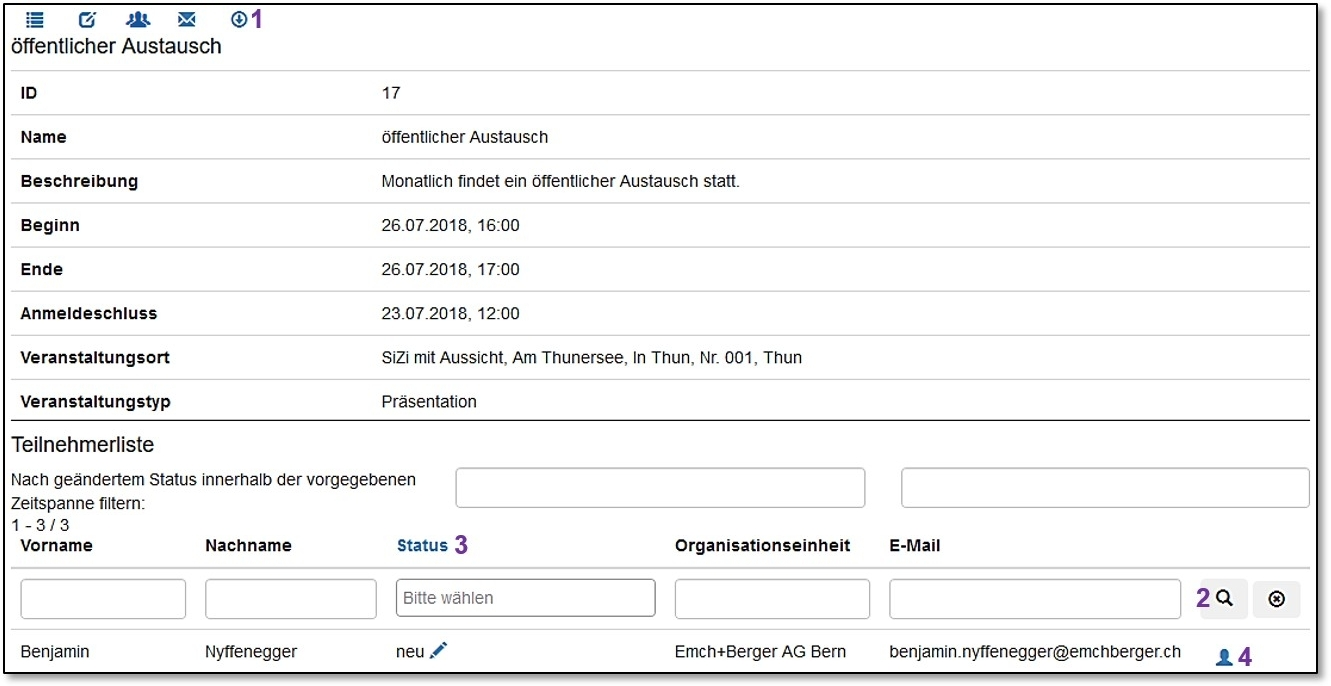
\includegraphics[width=1\linewidth]{../chapters/10_CRM/pictures/10-2-2_Teilnehmerliste_exportieren.jpg}}
\caption{Teilnehmerliste exportieren}
% \label{fig:speciation}
\end{figure}

Ebenso können Sie im Betrachtungsmodus 
\includegraphics[height=12pt]{/Icons/Lupe.jpg} in der Teilnehmerliste nach den verschiedenen Feldern (Vorname, Nachnamen, Status, Organisationseinheit und Email) suchen \col{(2)} und die Einträge nach dem Status sortieren \col{(3)} (Klick auf den blauen Statustitel). Verwenden Sie das Personensymbol 
\includegraphics[height=12pt]{/Icons/Person.jpg} \col{(4)} gelangen Sie direkt in die Adressliste, um den Eintrag einer Person zu ändern. Um von der Adressliste wieder zum CRM zurückzukehren, schliessen Sie nach dem Speichern (Klick auf 'Übernehmen') das zusätzlich geöffnete Browserfenster.


\pagebreak
\subsubsection{Vordefinierte Teilnehmerlisten erstellen}
\label{bkm:Ref2018072301}

Klicken Sie im Menü links auf 'Customer Relationship Management' und auf den Unterpunkt 'Teilnehmerlisten'. Es erscheint folgende Übersicht:

\begin{figure}[H]
\center{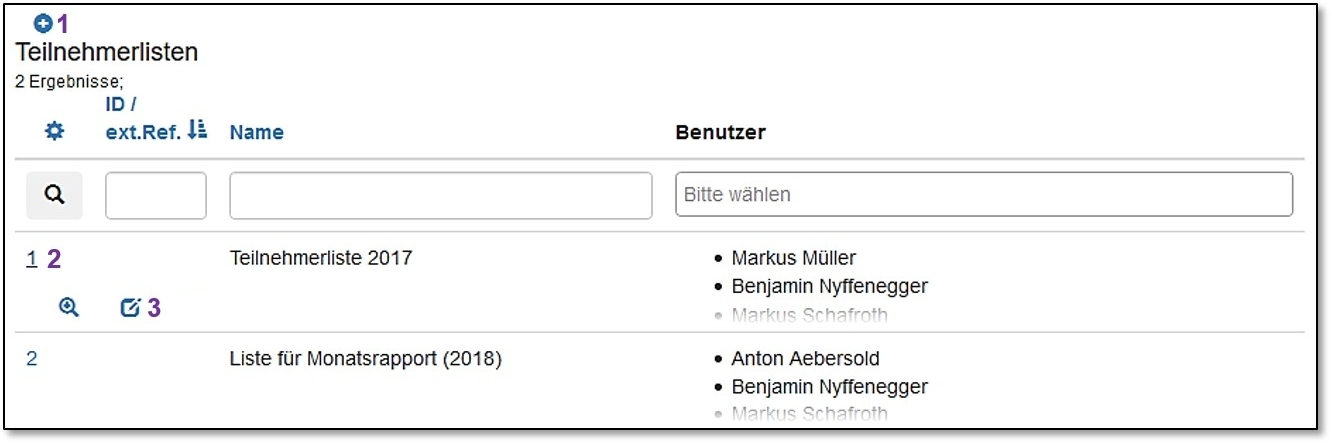
\includegraphics[width=1\linewidth]{../chapters/10_CRM/pictures/crm_TeilnehmerlistenUebersicht.jpg}}
\caption{Teilnehmerliste Übersicht}
% \label{fig:speciation}
\end{figure}

Nun können Sie mit dem Plussymbol 
\includegraphics[height=12pt]{/Icons/Plussymbol.jpg} \col{(1)} einen neue Liste erstellen. 

\vspace{\baselineskip}

Geben Sie der neuen Teilnehmerliste einen passenden Namen und wählen Sie die gewünschten Teilnehmer aus:

\begin{figure}[H]
\center{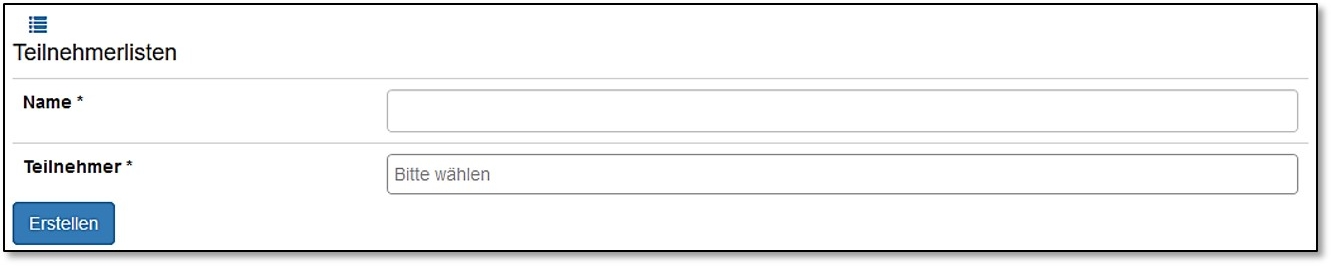
\includegraphics[width=1\linewidth]{../chapters/10_CRM/pictures/crm_Teilnehmerliste_erstellen.jpg}}
\caption{Teilnehmerliste erstellen}
% \label{fig:speciation}
\end{figure}

Mit 'Erstellen' schliessen Sie diesen Vorgang ab. 

\vspace{\baselineskip}

Eine bestehende Liste bearbeiten Sie, indem Sie auf die ID \col{(2)} klicken und dann mittels Bearbeiten-Symbol 
\includegraphics[height=12pt]{/Icons/Bearbeiten.jpg} \col{(3)} das Formular öffnen:

\begin{figure}[H]
\center{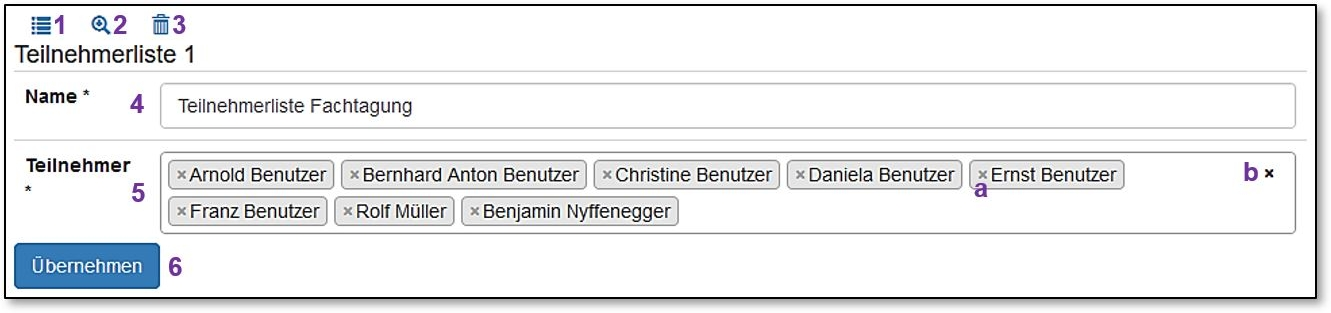
\includegraphics[width=1\linewidth]{../chapters/10_CRM/pictures/crm_Teilnehmerliste_bearbeiten.jpg}}
\caption{Teilnehmerliste bearbeiten}
% \label{fig:speciation}
\end{figure}

Verlassen Sie das Bearbeitungsfenster mit Klick auf das Listensymbol 
\includegraphics[height=12pt]{/Icons/Listensymbol_zurueck.jpg} \col{(1)} oder wechseln Sie in den Ansichtsmodus mittels 
\includegraphics[height=12pt]{/Icons/Lupe.jpg} \col{(2)}. Eine bestehende und nicht mehr verwendete Teilnehmerliste können Sie mit Klick auf das Mülltonnensymbol 
\includegraphics[height=12pt]{/Icons/Muelltonne.jpg} \col{(3)} löschen.\\
Die Felder 'Name*' \col{(4)} und 'Teilnehmer*' \col{(5)} sind Pflichtfelder, der Name der Teilnehmerliste können Sie nachträglich immer wieder anpassen. Überzählige Teilnehmer können Sie mit Klick auf das Kreuzchen \col{(a)} löschen. Wollen Sie sämtliche Teilnehmer aus der Liste entfernen, klicken Sie auf das Kreuzchen am Ende des Feldes \col{(b)}. Sämtliche Änderungen werden mit dem 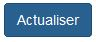
\includegraphics[height=12pt]{/Icons/B_Uebernehmen.jpg}-Button \col{(6)} gespeichert.

\vspace{\baselineskip}

\textbf{Teilnehmerliste aus der Adressliste erstellen}
\label{bkm:Ref20190313001}

\vspace{\baselineskip}

In der Adressliste können Sie mit wenigen Klicks neue Teilnehmerlisten erstellen. Wechseln Sie in das Menü 'Adressliste' und das Untermenü 'Personen':

\begin{figure}[H]
\center{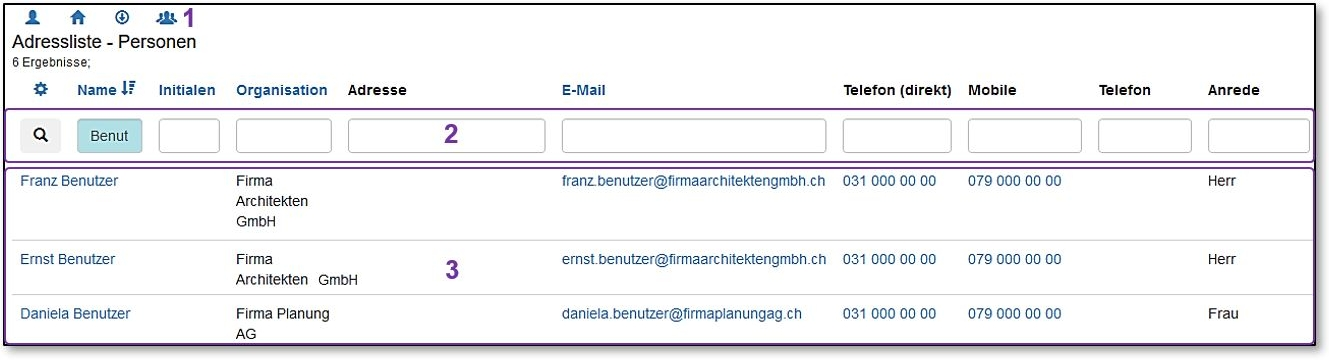
\includegraphics[width=1\linewidth]{../chapters/10_CRM/pictures/crm_Teilnehmerliste_ausAdressliste.jpg}}
\caption{Teilnehmerliste aus der Adressliste erstellen}
% \label{fig:speciation}
\end{figure}

Suchen Sie mittels dem Filter \col{(2)} die gewünschten Adressen. Alle angezeigten Personen / Adressen \col{(3)} werden in die Teilnehmerliste übernommen. Klicken Sie auf das Personen-Icon 
\includegraphics[height=12pt]{/Icons/Gruppe.jpg}-Button \col{(1)}.
Die neue Teilnehmerliste wird geöffnet:

\begin{figure}[H]
\center{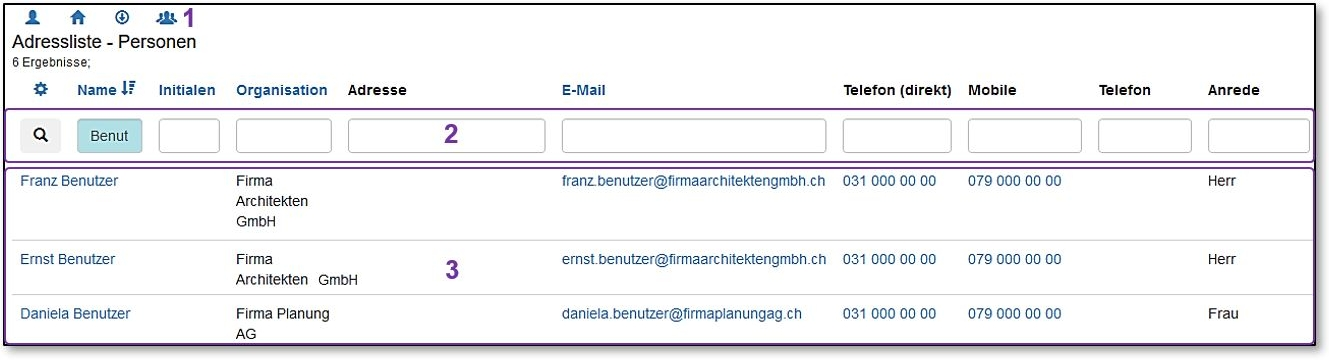
\includegraphics[width=1\linewidth]{../chapters/10_CRM/pictures/crm_Teilnehmerliste_ausAdressliste.jpg}}
\caption{Neue Teilnehmerliste aus der Adressliste}
% \label{fig:speciation}
\end{figure}

Geben Sie der Adressliste den gewünschten Namen und nehmen Sie die nötigen Änderungen vor. Der Vorgang wird mittels Klick auf den 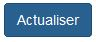
\includegraphics[height=12pt]{/Icons/B_Uebernehmen.jpg}-Button \col{(6)} abgeschlossen.

\vspace{\baselineskip}

\textbf{Hinweis:} In der Adressliste können benutzerdefinierte Felder eingerichtet werden. Diese sind gerade beim Erstellen von Teilnehmerliste für Veranstaltungen hilfreich. Haben Sie regelmässig einen Geschäftsanlass kann dieser als Zusatzfeld in der Adressliste aufgeführt werden. Alle eingeladenen Personen erhalten in diesem Feld beispielsweise ein 'Ja'. Soll nun eine neue aktuelle Teilnehmerliste erstellt werden, filtern Sie unter diesem Zusatzfeld sämtliche Personen heraus, welche in diesem Eintrag 'Ja' hinterlegt haben.

\vspace{\baselineskip}

% \pagebreak
\textbf{Selbstregistrierung durch Teilnehmer}
\label{bkm:Ref2018072302}

Wenn Sie die Option 'Selbstregistrierung durch Teilnehmer' wählen, erscheint im Ansichtsmodus der Einladung der Link für die Registrierungsseite:

\begin{figure}[H]
\center{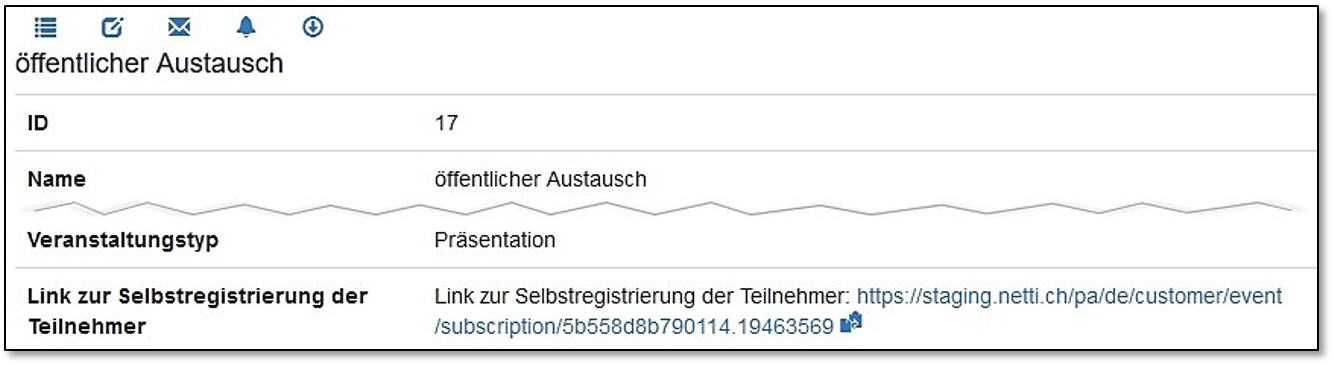
\includegraphics[width=1\linewidth]{../chapters/10_CRM/pictures/crm_LinkSelbstregistrierung.jpg}}
\caption{Link für die Selbstregistrierung}
% \label{fig:speciation}
\end{figure}

Folgende Maske erscheint:

\begin{figure}[H]
\center{\includegraphics[width=.5\linewidth]{../chapters/10_CRM/pictures/crm_Anmeldung.jpg}}
\caption{Link für die Selbstregistrierung}
% \label{fig:speciation}
\end{figure}

\pagebreak
\subsubsection{Einladungsseite gestalten (Online-Flyer)}
\label{bkm:Ref112017101}

\begin{wrapfigure}[3]{r}{9cm}   
  \vspace{-30pt}      
  \begin{center}
    \includegraphics[width=1\linewidth]{../chapters/10_CRM/pictures/crm_Einladung_gestalten_Link.jpg}
  \end{center}
  \vspace{-20pt}
  \caption{Einladungsseite gestalten}
  \vspace{-10pt}
\end{wrapfigure}

Klicken Sie im Bearbeitungsmodus der Einladung auf den blauen Text 'Anmeldeseite bearbeiten' \col{(1)}. 

% \begin{figure}[H]
% \center{\includegraphics[width=1\linewidth]{../chapters/10_CRM/pictures/crm_Einladung_gestalten_Link.jpg}}
% \caption{Einladungsseite gestalten}
% \end{figure}

\vspace{2cm}

Nun wird eine leere Editierseite der Onlineeinladung geöffnet:

\begin{figure}[H]
\center{\includegraphics[width=1\linewidth]{../chapters/10_CRM/pictures/10-2-3_Leere_Einladung.jpg}}
\caption{Leere Einladungsseite}
% \label{fig:speciation}
\end{figure}

Mit dem Stiftsymbol \includegraphics[height=12pt]{/Icons/Stift.jpg} können Sie nun die verschiedenen Bereiche gestalten. Mit dem Kreuzsymbol \includegraphics[height=12pt]{/Icons/Kreuzchen_b.jpg} können Sie Bereiche löschen.
Die grossen Icons stehen für einen Titel \col{(1)}. Mit Klick auf den Stift \includegraphics[height=12pt]{/Icons/Stift.jpg} öffnet sich ein kleines Textfeld, in welchem Sie den Titel des Bereiches eingeben und mit dem Gutzeichen \includegraphics[height=12pt]{/Icons/Gutzeichen.jpg} speichern können.
Mit Klick auf den Stift \includegraphics[height=12pt]{/Icons/Stift.jpg} für die Beschreibung \col{(2)} öffnet sich ein ausführliches Editierfenster, in welchem Sie den Text nach Belieben formatieren können (siehe unten). Unterhalb des Textes 'Platzhalter für Bild, editieren mit Bleistift unter diesem Satz' können Sie mit Klick auf den Stift \includegraphics[height=12pt]{/Icons/Stift.jpg} ein Bild hochladen, indem Sie auf 'Durchsuchen' klicken und das gewünschte Bild auswählen und mit dem Gutzeichen \includegraphics[height=12pt]{/Icons/Gutzeichen.jpg} bestätigen. 

\vspace{\baselineskip}

Die Anmeldung \col{(4)} können Sie mit Klick auf den blauen Pfeil nach Links (oder dann wieder rechts) platzieren.

\begin{figure}[H]
\center{\includegraphics[width=.7\linewidth]{../chapters/10_CRM/pictures/10-2-3_Text_formatieren.jpg}}
\caption{Text formatieren}
% \label{fig:speciation}
\end{figure}

\subsubsection{Einladungen versenden}

Im Betrachtungs- oder Bearbeitungsmodus der Veranstaltungen gelangen Sie mit Klick auf das Briefsymbol \includegraphics[height=12pt]{/Icons/Briefsymbol.jpg} auf die Bearbeitungsseite der Einladungsvorlage. Auf dieser Seite sehen Sie nochmals die terminlichen Eckdaten im Überblick. Zudem gelangen Sie mit dem roten Bearbeitungs- und Lupensymbol \col{(1)} auch von hier zur Bearbeitungsseite der Onlineeinladung, respektive der Betrachtungsseite der Onlineeinladung. \\

\begin{figure}[H]
\center{\includegraphics[width=.8\linewidth]{../chapters/10_CRM/pictures/10-2-4_Einladungsvorlage.jpg}}
\caption{Emailvorlage}
% \label{fig:speciation}
\end{figure}

Ihnen wird ein Einladungstext vorgeschlagen, welcher Sie aber nach Belieben auch anpassen können. Dazu klicken Sie auf das Bearbeitungssysmbol \includegraphics[height=12pt]{/Icons/Bearbeiten.jpg} \col{(2)}. Im Folgenden können Sie den vorgeschlagenen Text der Einladung anpassen (siehe unten). Entspricht der Einladungstext Ihren Wünschen, können Sie die Einladung mit Klick auf den Button 'Einladung versenden' \col{(3)} versenden. Die Einladung wird nur an Personen verschickt, welche den Status 'neu' haben.

\begin{figure}[H]
\center{\includegraphics[width=1\linewidth]{../chapters/10_CRM/pictures/10-2-4_Einladungsvorlage_bearbeiten.jpg}}
\caption{Emailvorlage bearbeiten}
% \label{fig:speciation}
\end{figure}

Nun können Sie den Einladungstext \col{(3)} ändern. Mit Klick auf das Diskettensymbol \includegraphics[height=12pt]{/Icons/Diskette.jpg} \col{(1)} werden die Einstellungen gespeichert; mit Klick auf das blaue Kreuzchen \includegraphics[height=12pt]{/Icons/Kreuzchen_b.jpg} \col{(2)} werden die Änderungen verworfen.\\
Zur Hilfestellung sehen Sie rechts die Übersicht der Platzhalter für die Einladung \col{(4)}. Bevor Sie die Einladung versenden \col{(5)}, speichern \col{(1)} oder verwerfen \col{(2)} Sie die Änderungen.

\vspace{\baselineskip}

\textbf{Hinweis:} Falls Sie nicht auf den Button 'Einladung versenden' drücken können (er wird etwas aufgehellt dargestellt - siehe oben \col{(5)}), stimmt etwas mit den Angaben für die Einladung nicht. Beispielsweise wurde ein Datum gewählt, das in der Vergangenheit liegt.

\vspace{\baselineskip}

Sobald eine Einladung verschickt wurde (an alle Empfänger mit Status 'neu'), erscheint nun bei den Personen rechts ein Fliegersymbol \includegraphics[height=12pt]{/Icons/Versandsymbol.jpg} \col{(1)}.

\begin{figure}[H]
\center{\includegraphics[width=1\linewidth]{../chapters/10_CRM/pictures/crm_Mail_versenden.jpg}}
\caption{Neue Email mit Einladungstext versenden}
% \label{fig:speciation}
\end{figure}

Mit Klick darauf wird eine neue Email geöffnet, welche den Einladungstext enthält.

\subsubsection{Status der Einladungen}

Mit jedem Schritt der Einladung verändert sich der Status der Teilnehmer.

Folgende Statis werden verwendet:

\begin{wrapfigure}[11]{l}{5.2cm}   % [x] Wie manche Zeile soll sich um die Grafik "brechen"
  \vspace{-10pt}      % Grundwert war 20; mit 30 schön oben beim Text ausgerichtet
  \begin{center}
    \includegraphics[width=.9\linewidth]{../chapters/10_CRM/pictures/10-2-5_Status.jpg}
  \end{center}
  \vspace{-20pt}
  % \caption{Neue Veranstaltung anlegen}
  \vspace{-10pt}
\end{wrapfigure}


\textbf{Überblick Statussystem:}

\textbf{neu:} Wird eine neue Veranstaltung erstellt und Teilnehmer hinzugefügt, erhalten diese den Status 'neu'. Eine Einladung wird nur an Teilnehmer mit Status 'neu' versendet.\\
\textbf{eingeladen:} Wurde die Einladung versendet, erhalten die Teilnehmer den Status 'eingeladen'.\\
\textbf{erinnert:} Teilnehmer, welche nicht reagiert haben, können erinnert werden.\\
\textbf{angemeldet:} Teilnehmer, welche sich über die Einladungswebseite angemeldet haben, erhalten den Status 'angemeldet'.\\
\textbf{teilgenommen:} Der Anlass hat stattgefunden und die teilgenommenen Teilnehmer erhalten den Status 'teilgenommen'.\\
\textbf{nachher kontaktiert:} Zum Einholen eines Feedbacks werden Teilnehmer nach dem Anlass kontaktiert. Um eine Übersicht über die Teilnehmer zu erhalten, welche bereits kontaktiert wurden, wird dieser Status gesetzt.\\
\textbf{abgemeldet:} Über die Webseite oder auf anderem Weg abgemeldete Teilnehmer erhalten den Status 'abgemeldet'.

\vspace{\baselineskip}

\textit{Status manuell bearbeiten:} Es ist möglich, einen Status eines Teilnehmers auch manuell zu ändern. Hat sich ein Teilnehmer beispielsweise nicht über die Einladungswebseite, sondern per Telefon angemeldet, kann die Administration mit Klick auf das Stiftsymbol \includegraphics[height=12pt]{/Icons/Stift.jpg} ein Status manuell anpassen. Diese Mutation funktioniert im Bearbeitungs- oder Übersichtsmodus der Veranstaltung.

\vspace{\baselineskip}

\textbf{Beachten Sie folgende Gegebenheiten beim Versand von Anmeldungen:} 

\vspace{\baselineskip}

\begin{compactitem}
	\item Erstmalige Anmeldungen müssen mittels Status 'neu' und dem Button 'Einladung versenden' ausgelöst werden.
	\item In der Folge erscheint bei der Teilnehmerliste das \includegraphics[height=12pt]{/Icons/Versandsymbol.jpg}-Symbol für persönliche Nachrichten.
	\item Soll mittels persönlicher Nachricht (\includegraphics[height=12pt]{/Icons/Versandsymbol.jpg}-Symbol) ein An-/Abmeldelink erneut verschickt werden, erfordert dies mindestens den Status 'eingeladen'. (Mit Status 'neu' wird der verschickte Link nicht funktionieren).
	\item Achten Sie bei der Anmeldung auf den Anmeldeschluss: wird dieser Termin erreicht, funktioniert die Anmeldeseite nicht mehr.
\end{compactitem}

\pagebreak
\subsubsection{Anmeldung und Abmeldung durch die Teilnehmer}

Die Teilnehmer erhalten die Einladung per Mail. In der Einladungsmail befindet sich ein Link auf die zuvor erstellte Einladungsseite. Diese Seite entspricht einem Flyer mit allen nötigen Angaben. Über diese Einladungsseite können die Teilnehmer mit einem Klick ihre Anmeldung bestätigen oder sich allenfalls auch abmelden. Nach dem entsprechenden Klick durch den Teilnehmer wird der Status des jeweiligen Teilnehmers im CUBE PA CRM automatisch aktualisiert. 

\begin{figure}[H]
\center{\includegraphics[width=1\linewidth]{../chapters/10_CRM/pictures/10-2-6_AnAbmeldungUebersicht.jpg}}
\caption{Übersicht An- und Abmeldungen}
% \label{fig:speciation}
\end{figure}

In der Veranstaltungsübersicht \includegraphics[height=12pt]{/Icons/Lupe.jpg} sehen Sie die komplette Teilnehmerliste. Mit Klick auf das Downloadsymbol \includegraphics[height=12pt]{/Icons/ListeGenerieren.jpg} oben in der Mitte des Fensters können Sie die gefilterten / angezeigten Teilnehmer als Liste im Excel-Format abspeichern. Filtern Sie unter \col{(2)} die Einträge nach dem Datum. Mit Klick in eines der beiden Datumfenster öffnet sich eine Kalenderansicht. Wählen Sie den gewünschten Tag aus. \\
Bei \col{(3)} sehen Sie wie viele Teilnehmer sich auf der Liste befinden. In den weiteren Feldern \col{(4)} können Sie innerhalb der Teilnehmerliste nach Einträgen suchen / filtern. Mit Klick auf den Stift \includegraphics[height=12pt]{/Icons/Stift.jpg} \col{(5)} ändern Sie den Status eines Teilnehmers. Wollen Sie die Person in der Adressliste mutieren, klicken Sie auf das Personensymbol \includegraphics[height=12pt]{/Icons/Person.jpg} \col{(6)}. Ein zusätzliches Browserfenster wird geöffnet. Nach dem Ändern der gewünschten Feldern und Klick auf 'Übernehmen' können Sie das zusätzlich geöffnete Browserfenster wieder schliessen. 

\pagebreak

\textbf{Beispiel einer Einladung:}
\begin{figure}[H]
\center{\includegraphics[width=1\linewidth]{../chapters/10_CRM/pictures/10-2-6_Beispiel.jpg}}
% \caption{Übersicht An- und Abmeldungen}
% \label{fig:speciation}
\end{figure}

% \subsubsection{Bestehende Veranstaltungen betrachten und bearbeiten}

% Veranstaltung löschen
% Text x

